\documentclass{beamer} 
\usepackage{beamerthemesplit} 
\usepackage{wrapfig} 
\usepackage{verbatim} 
\usetheme{SPbGU} 
\usepackage{pdfpages} 
\usepackage{amsmath} 
\usepackage{cmap}
\usepackage{array} 
\usepackage[T2A]{fontenc} 
\usepackage[utf8]{inputenc} 
\usepackage[english,russian]{babel} 
\usepackage{indentfirst} 
\usepackage{amsmath} 
\usepackage{tikz} 
\usepackage{multirow} 
\usepackage[noend]{algpseudocode} 
\usepackage{algorithm} 
\usepackage{algorithmicx} 
\usetikzlibrary{shapes,arrows} 
\usepackage{fancyvrb} 
\usepackage{tikz} 
\usepackage{pgfplots} 
\usepackage{sidecap} 
\usepackage{soul}
\usepackage{xcolor}
\usepackage{tabu}
\usepackage{tikz}
\usetikzlibrary{calc}
\usepackage{zref-savepos}
\usepackage{colortbl}
\pgfplotsset{compat=1.9} 
\newtheorem{rutheorem}{Теорема} 
\newtheorem{ruproof}{Доказательство} 
\newtheorem{rudefinition}{Определение} 
\newtheorem{rulemma}{Лемма} 
\beamertemplatenavigationsymbolsempty 

\newcounter{NoTableEntry}
\renewcommand*{\theNoTableEntry}{NTE-\the\value{NoTableEntry}}

\newcommand*{\strike}[2]{%
	\multicolumn{1}{#1}{%
		\stepcounter{NoTableEntry}%
		\vadjust pre{\zsavepos{\theNoTableEntry t}}% top
		\vadjust{\zsavepos{\theNoTableEntry b}}% bottom
		\zsavepos{\theNoTableEntry l}% left
		\hspace{0pt plus 1filll}%
		#2% content
		\hspace{0pt plus 1filll}%
		\zsavepos{\theNoTableEntry r}% right
		\tikz[overlay]{%
			\draw
			let
			\n{llx}={\zposx{\theNoTableEntry l}sp-\zposx{\theNoTableEntry r}sp-\tabcolsep},
			\n{urx}={\tabcolsep},
			\n{lly}={\zposy{\theNoTableEntry b}sp-\zposy{\theNoTableEntry r}sp},
			\n{ury}={\zposy{\theNoTableEntry t}sp-\zposy{\theNoTableEntry r}sp}
			in
			(\n{llx}, \n{lly}) -- (\n{urx}, \n{ury})
			;
		}% 
	}%
}

\title[]{Extended Context-Free Grammars Parsing with Generalized LL} 
% То, что в квадратных скобках, отображается в левом нижнем углу. 
\institute[SPbU]{ 
	Saint Petersburg University \\ 
	Programming Languages and Tools Lab, JetBrains} 

% То, что в квадратных скобках, отображается в левом нижнем углу. 
\author[Artem Gorokhov]{Artem Gorokhov} 
\date{March 4,2017} 

\begin{document} 
	
	\definecolor{red}{RGB}{255,0,0} 
	
	\begin{frame} 
		\begin{columns} 
			\begin{column}{6.1cm}
				\begin{center} 
					{
\includegraphics[width=2.5cm]{pictures/jetbrains_logo.jpg}} 
				\end{center}
			\end{column}
			\begin{column}{6.1cm}
				\begin{center} 
					{
\includegraphics[width=2.5cm]{pictures/SPbGU_Logo.png}} 
				\end{center}
			\end{column}
			\end{columns}
		 
		\titlepage 
		%Hello, My name is Artem
		%Im from Jetbrains programming languages and tools laboratory
		%I would like to tell you about 
		%Extended Context-Free Grammars Parsing with Generalized LL Algorithm
	\end{frame}

	\begin{frame}
		\begin{center} 
			{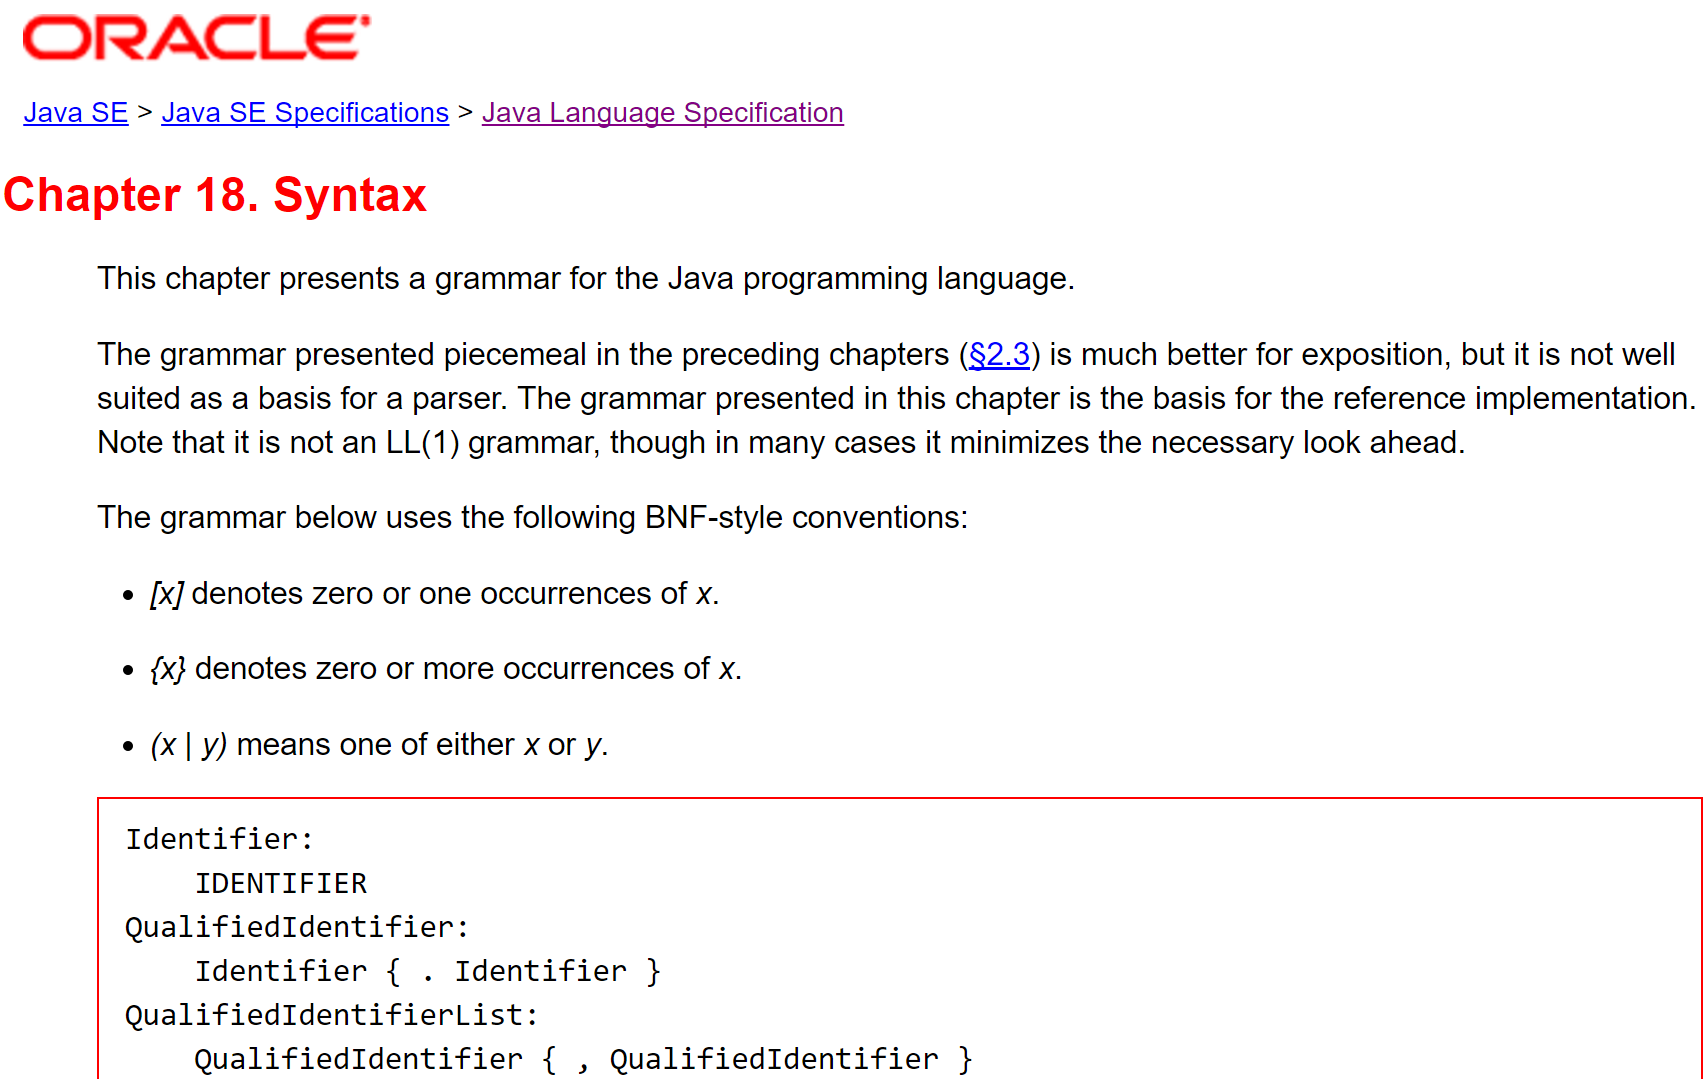
\includegraphics[width=12cm]{pictures/java_grammar.png}} 
		\end{center}
	\end{frame}

	\begin{frame} 
		\frametitle{Extended Context-Free Grammar}
		\begin{center}
			{$\begin{aligned}
				S\ =&\ a\ M^* \\
				M\ =&\ a?\ (B\ K)^+ \\
				|&\ u\ B \\
				B\ =&\ c\ |\ \varepsilon
				\end{aligned}$}
		\end{center}
	\end{frame}
	
	\begin{frame}
		\begin{columns}
			\begin{column}{6.1cm}
				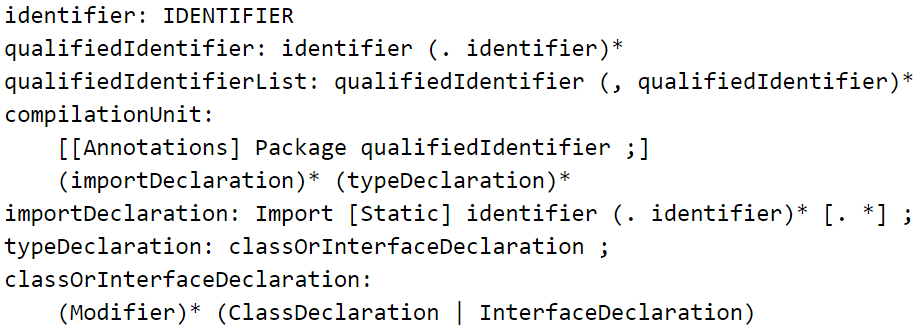
\includegraphics[width=6cm]{pictures/java_before.png}
			\end{column}
			\begin{column}{.7cm}
				$ \Longrightarrow $
			\end{column}
			\begin{column}{5cm}
				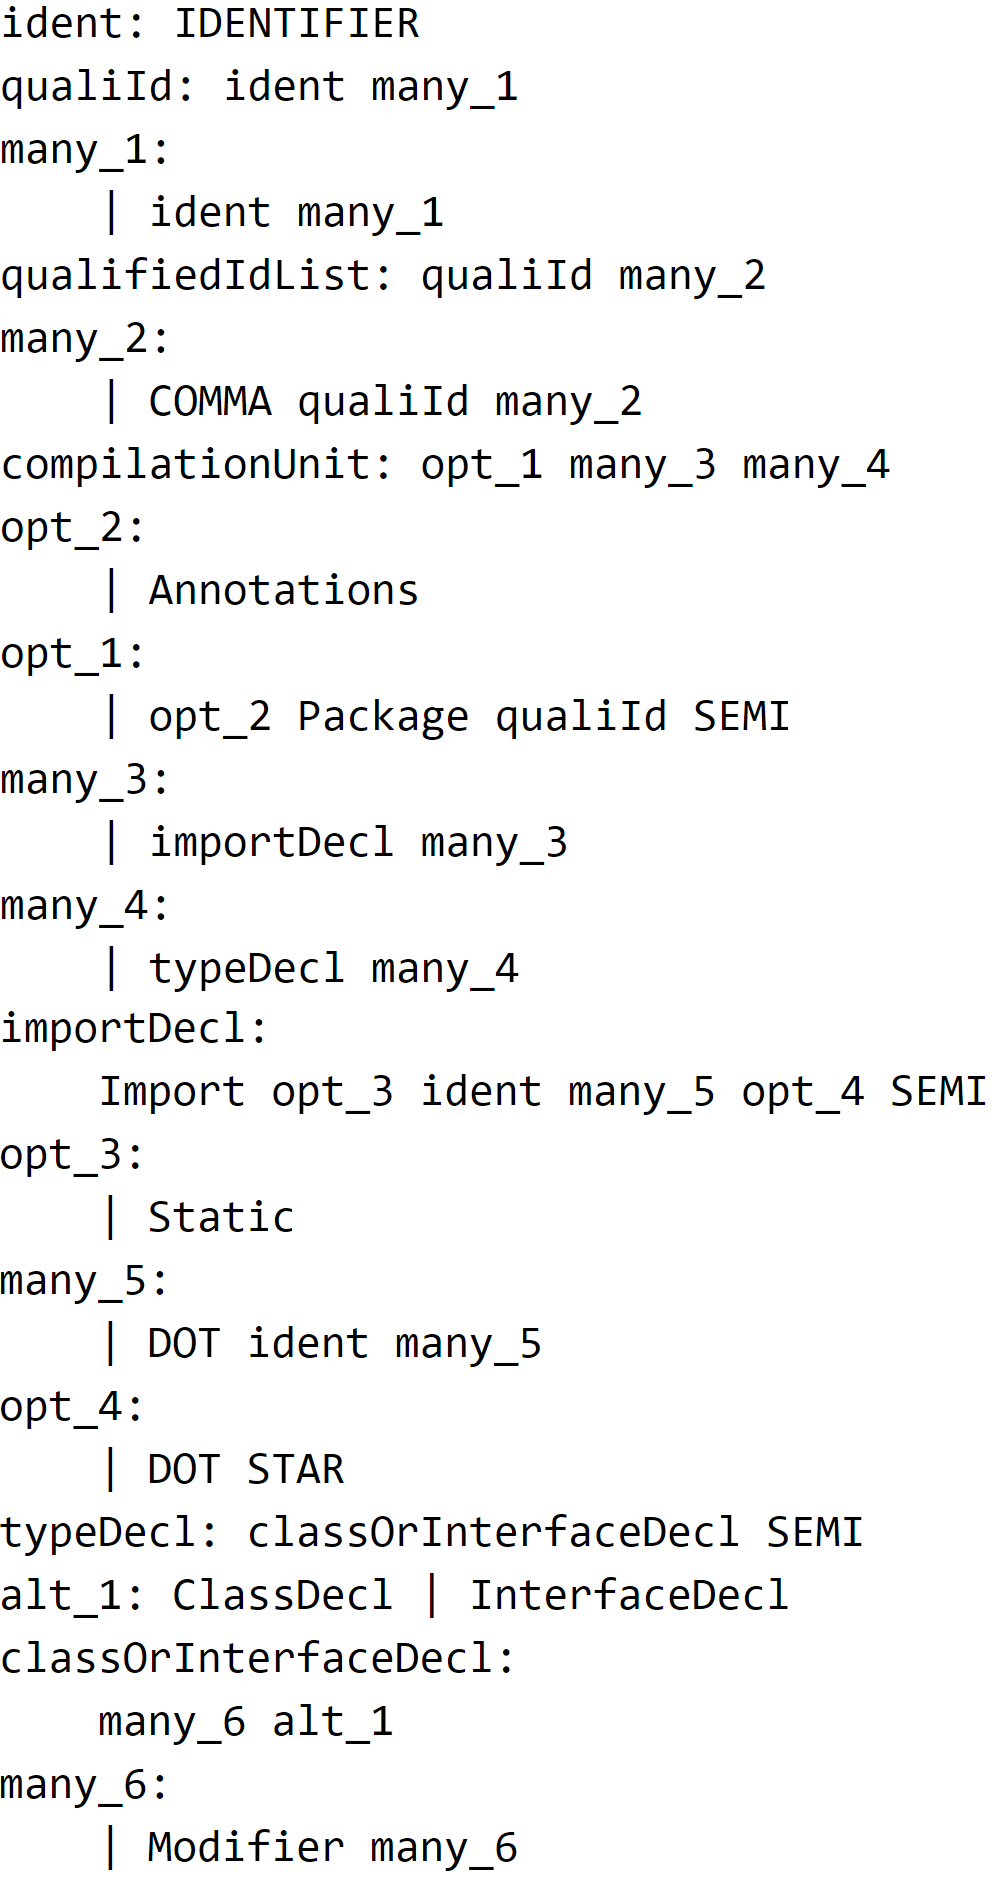
\includegraphics[width=4.8cm]{pictures/java_after.png}
			\end{column}
	    \end{columns}
	\end{frame}

\begin{frame}
	\begin{center} 
		\only<1>{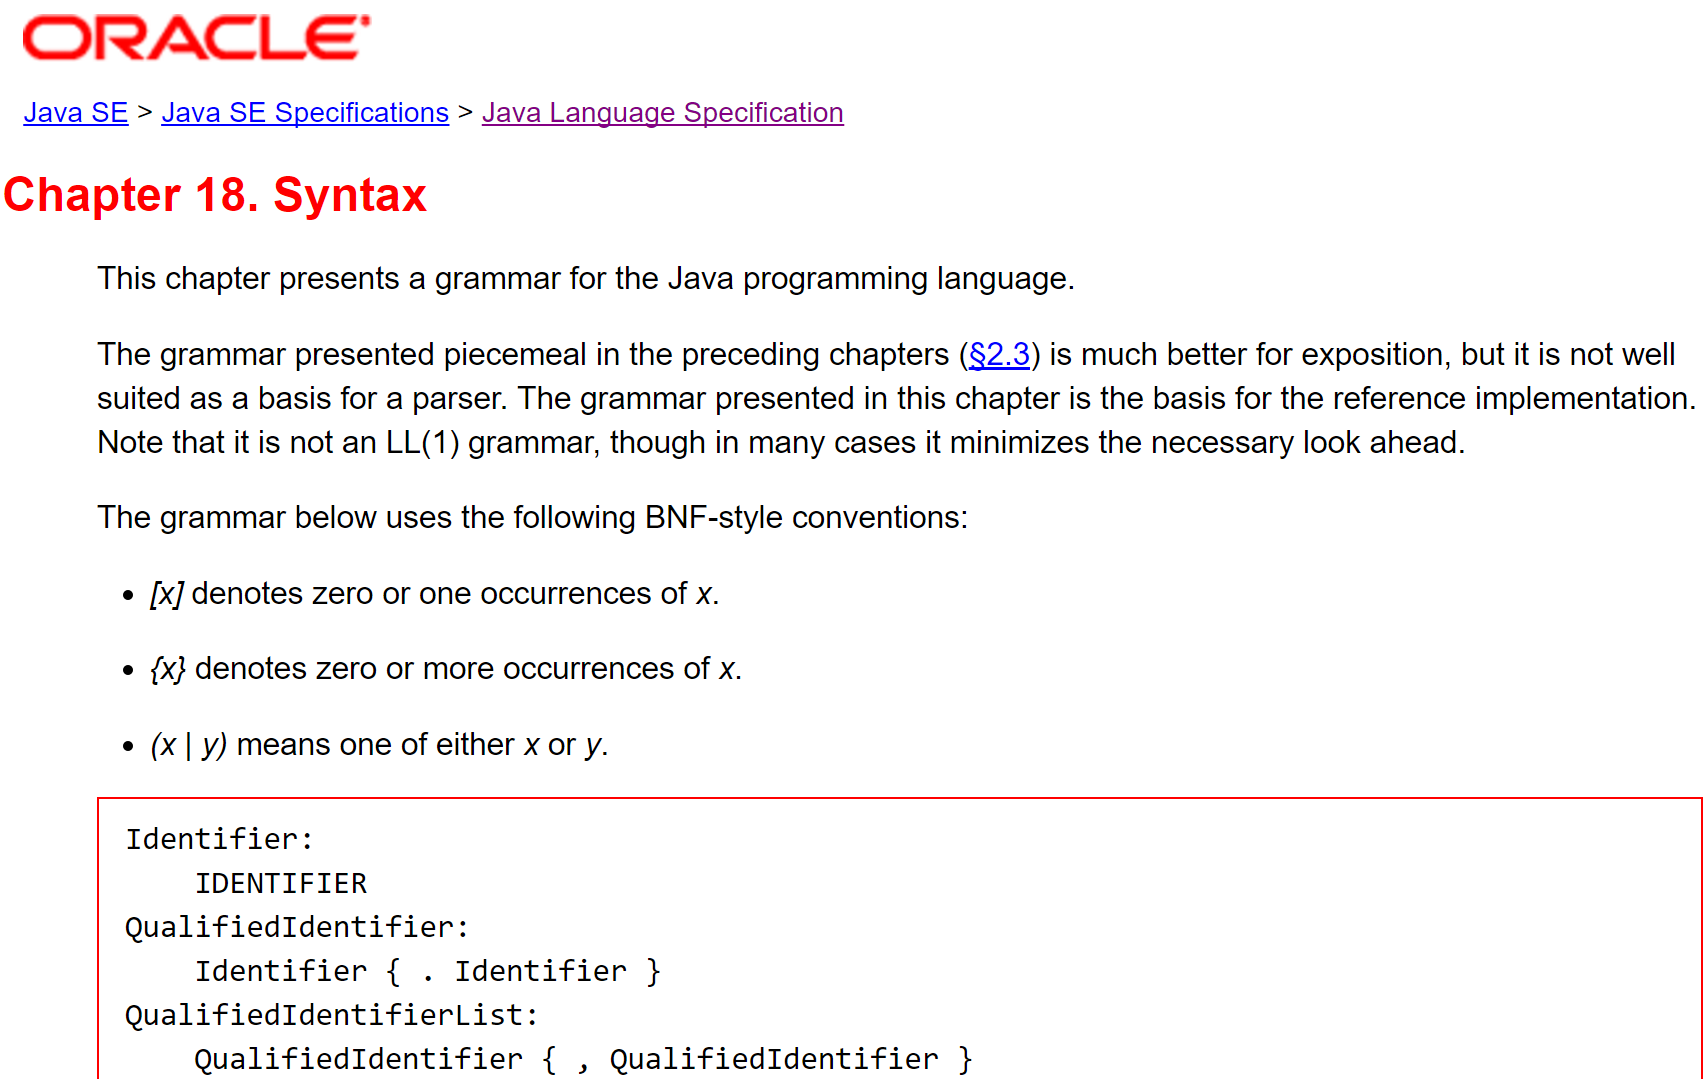
\includegraphics[width=12cm]{pictures/java_grammar.png}} 
		\only<2>{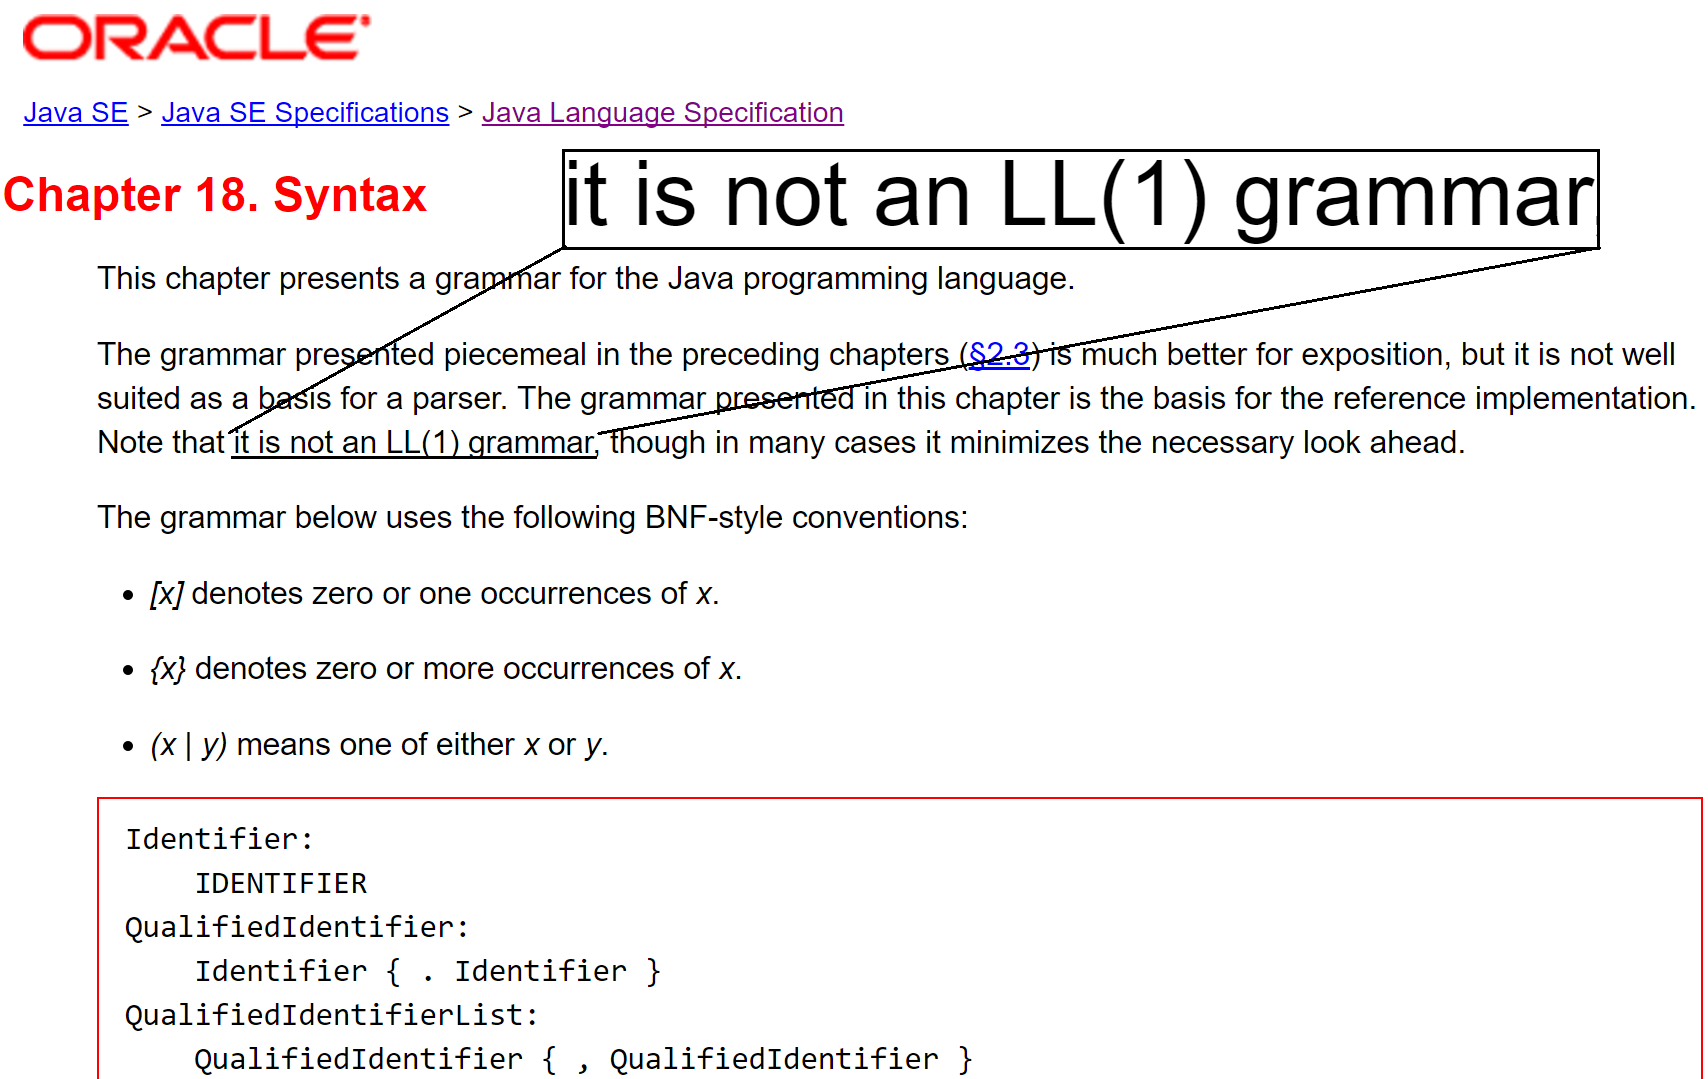
\includegraphics[width=12cm]{pictures/java_grammar_2.png}} 
	\end{center}
\end{frame}

	

	\begin{frame} 
		\frametitle{Existing solutions} 
		\begin{itemize}
			\item<1-> ANTLR, Yacc, Bison
			 \begin{itemize}
			 	\item<2-> Can't use ECFG without transformation
			 	\item<2-> Admit only subclass of Context-Free languages (LL(k), LR(k))
			 \end{itemize} 
			\item<3-> Some research on ECFG parsing
			\begin{itemize}
				\item<4-> No tools
				\item<4-> LL(k), LR(k)
			\end{itemize}
			\item<5-> \only<5-6>{Generalized LL}\only<7>{\textbf{Generalized LL}}
			\begin{itemize}
				\item<6-> Admit arbitrary CFG (including ambiguous)
				\item<6-> Can't use ECFG without transformation
			\end{itemize}
		\end{itemize}
	\end{frame}

	\begin{frame} 
		\frametitle{Automata and ECFGs}
		
		\begin{columns}
			\begin{column}{4cm}
				Grammar $G_0$\\
				\vspace{10pt}
				$
				\begin{array}[b]{rl}
				S = a^{*} S\ b? \ | \ c \ \ \ \ \ \ \ \ \  \Longrightarrow
				\end{array}
				$
			\end{column}
			\begin{column}{3.3cm}
				RA for grammar $G_0$\\
				\vspace{10pt}
				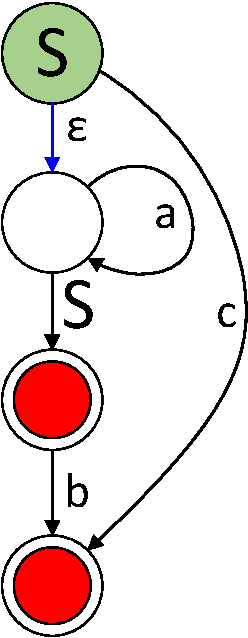
\includegraphics[width=2.5cm]{pictures/G0initialAutomaton.pdf}
			\end{column}
		\end{columns}
	\end{frame}

	\begin{frame} 
		\frametitle{Recursive Automata Minimization}
		\vspace{-12pt}
		\begin{center}
			%\begin{tabular}{c}
			{Grammar $G_1$\\
			\vspace{5pt}
			$
			\begin{array}{rl}
			S =& K\ K\ K\ K\ K\ K \ |K\ a\ K\ K\ K\ K \\
			K =& S\ K\ |\ a\ K\ |\ a \\
			\end{array}
			$
			}
		    \\
		    \vspace{12pt}
		    Automaton for $G_1$
		    \\
		    \vspace{5pt}
		    {
				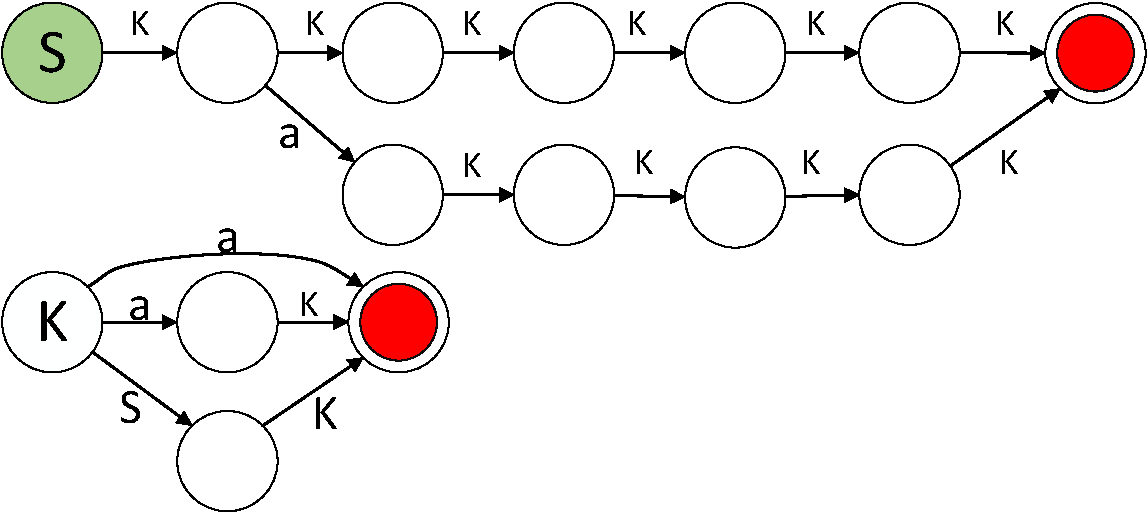
\includegraphics[width=7cm]{pictures/G1initial.pdf}
			}\\
			\vspace{8pt}
			Minimized automaton for $G_1$
			\\
			\vspace{5pt}
		    {
				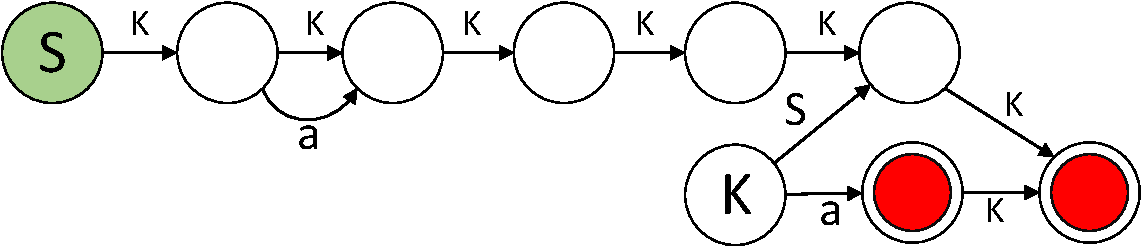
\includegraphics[width=7cm]{pictures/G1automaton.pdf}
			}
		\end{center}
	\end{frame}
	
	\begin{frame} 
		\frametitle{Derivation Trees for Recursive Automata}
		%\vspace{-40pt}
		\begin{columns}
			\begin{column}{3.7cm}
				%Grammar: $$ S : a^{+} S\ b? \ | \ c $$
				Input: $$aacb$$ \\
				\vspace{10pt}
				Automaton: \\
				\vspace{5pt}
				\begin{center}
					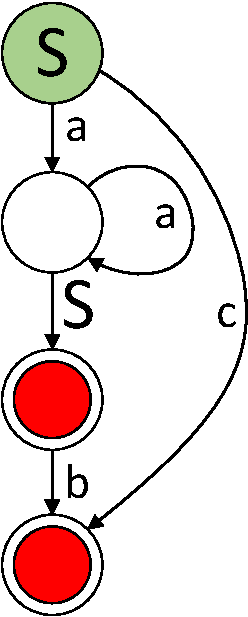
\includegraphics[width=2cm]{pictures/G0minimizedAutomaton.pdf}
				\end{center}
			\end{column}
		
     		\begin{column}{6cm}
     			\ \ Derivation trees:\\
     			\vspace{5pt}
     			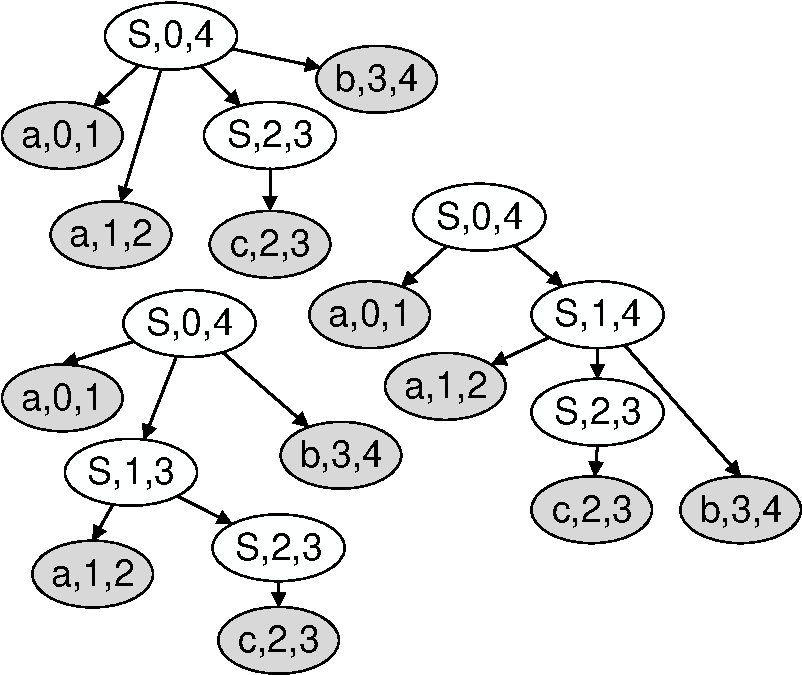
\includegraphics[width=7cm]{pictures/G0trees.pdf}
			\end{column}
		
		\end{columns}
	\end{frame}
	
	\begin{frame} 
		\frametitle{SPPF for Recursive Automata}
		\begin{columns}
			\begin{column}{5cm}
				%Grammar: $$ S : a^{+} S\ b? \ | \ c $$
				Input: $$aacb$$ \\
				\vspace{10pt}
				Automaton: \\
				\vspace{5pt}
				\begin{center}
					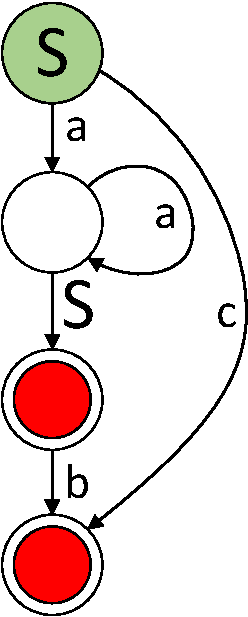
\includegraphics[width=2cm]{pictures/G0minimizedAutomaton.pdf}
				\end{center}
			\end{column}
			\begin{column}{6cm}
				Shared Packed Parse Forest: \\
				\vspace{10pt}
				\only<1>{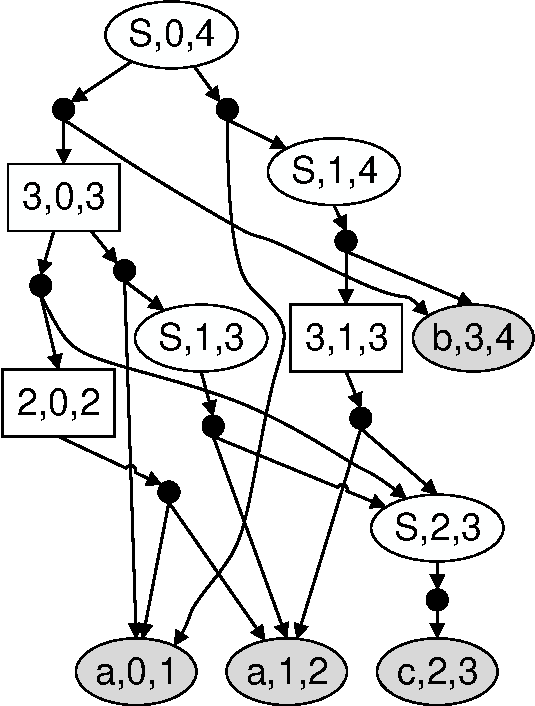
\includegraphics[width=5cm]{pictures/G0SPPF.pdf}}
				\only<2>{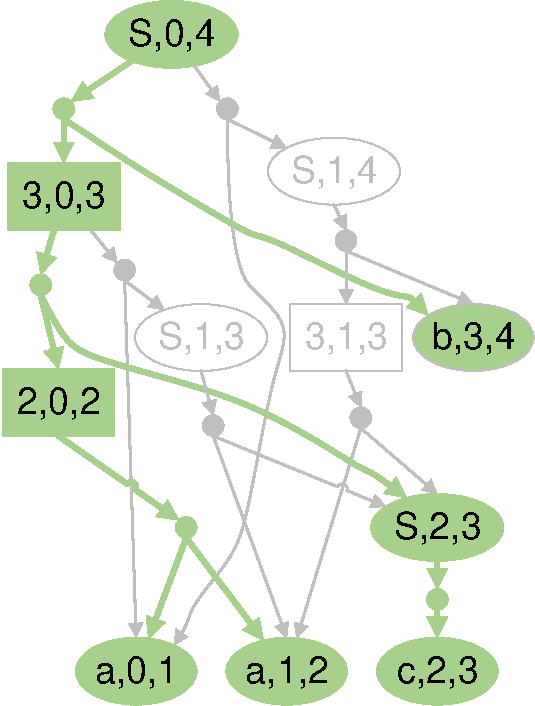
\includegraphics[width=5cm]{pictures/G0SPPF_1.pdf}}
				\only<3>{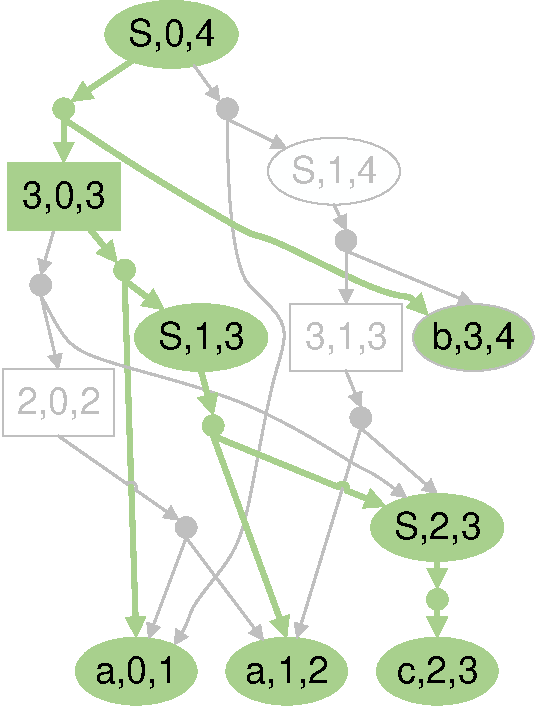
\includegraphics[width=5cm]{pictures/G0SPPF_2.pdf}}
				\only<4>{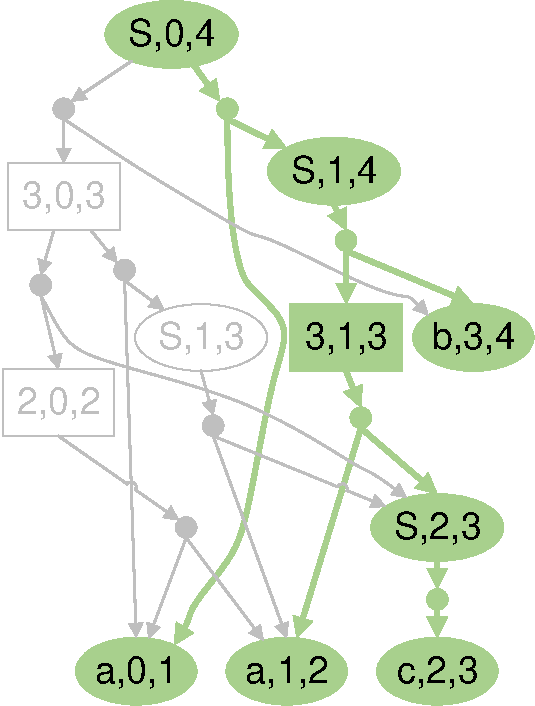
\includegraphics[width=5cm]{pictures/G0SPPF_3.pdf}}
			\end{column}
		\end{columns}
	\end{frame}
	
	\begin{frame} 
		\frametitle{Input processing}
		\begin{itemize}
			\item Descriptors queue
			\item Descriptor (G, i, U, T) uniquely defines parsing process state
			\begin{itemize}
				\item G - \only<1>{position in grammar}
						  \only<2>{\st{position in grammar}\ \  state of RA}
				\item i - position in input
				\item U - stack node
				\item T - current parse forest root
			\end{itemize}
		\end{itemize}
		
	\end{frame}
	\begin{frame} 
		\frametitle{Input processing}
		\begin{columns}
			\begin{column}{5cm}
				Input : \only<1-2>{$\ b c $}
						\only<3-7>{$\bullet\ b c $} 
						\only<8-11>{$b\bullet c $}
						\only<12->{$b c \bullet$} \\
				\vspace{15pt}
				Grammar: \\
				\vspace{5pt}
				\only<1>{$$
					S = \ (a\ |\ b\ |\ S)\ c?
					$$}
				\only<2->{$
				\begin{array}{rl}
				S =&\only<3,6>{\bullet} \ a\ C\_opt \\
				|&\only<4,7>{\bullet} \ b\only<8>{\bullet}\ C\_opt \\
				|&\only<5>{\bullet} \ S\ C\_opt \\
				C\_opt =& \only<9>{\bullet} \varepsilon \ | \only<10-11>{\bullet} \ c \only<12>{\ \bullet}\\
				\end{array}
				$}
			\end{column}
			
			\begin{column}{5cm}
				\only<3->{
				\only<8>{\vspace{50pt}}
				\only<12>{\vspace{44pt}}
				\begin{center}Descriptors queue\\\end{center}
				\begin{tabu}{|[3pt]c|[3pt]}
					\only<10>{$C\_opt =\bullet c$, 1, \dots, \dots \\ \hline}
					\only<11->{\cellcolor{green!25}{$C\_opt =\bullet c$, 1, \dots, \dots} \\ \hline}
					\only<11->{\st{$C\_opt =\bullet  \varepsilon$, 1, \dots, \dots} \\ \hline}
					\only<9-10>{$C\_opt =\bullet  \varepsilon$, 1, \dots, \dots \\ \hline}
					\only<5-10>{$S =\bullet \ S\ C\_opt$, 0, \dots, \dots \\ \hline}
					\only<11->{\st{$S =\bullet \ S\ C\_opt$, 0, \dots, \dots} \\ \hline}
					\only<3-4>{$\ \ \ \ \ \ \ \ \ \ \ \ \ \ \ \ \ \ \ \ \ \ \ \ \ \ \ \ \ \ \ \ \ \ $ \\}
					%\strike{|[3pt]c|}{quux} & A & B \\
					\only<4-6>{$S =\bullet \ b\ C\_opt$, 0, \dots, \dots \\ \hline}
					\only<7-10>{\cellcolor{green!25}{$S =\bullet \ b\ C\_opt$, 0, \dots, \dots} \\ \hline}
					\only<11->{\st{$S =\bullet \ b\ C\_opt$, 0, \dots, \dots} \\ \hline}
					\only<3>{$\ \ \ \ \ \ \ \ \ \ \ \ \ \ \ \ \ \ \ \ \ \ \ \ \ \ \ \ \ \ \ \ \ \ $ \\}
					\only<3-5>{$S =\bullet \ a\ C\_opt$, 0, \dots, \dots}
					\only<6>{\cellcolor{green!25}{$S =\bullet \ a\ C\_opt$, 0, \dots, \dots}}
					\only<7->{\st{$S =\bullet \ a\ C\_opt$, 0, \dots, \dots}}
				\end{tabu}
			}
		
			\only<8>{
				\vspace{20pt}
				\begin{center}
					\only<8>{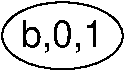
\includegraphics[width=2cm]{pictures/example_trees_b.pdf}}
				\end{center}				
			}
			\only<12>{
				\begin{center}
					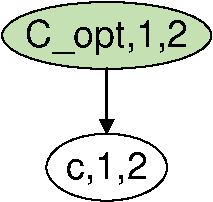
\includegraphics[width=2cm]{pictures/example_trees.pdf}
				\end{center}				
			}
			\end{column}
		    
		\end{columns}
	\end{frame}

	\begin{frame} 
		\frametitle{Input processing}
		\begin{columns}
			\begin{column}{5cm}
				Input : $\only<1>{\ \ }\only<2->{\bullet} \ b c $ \\
				\vspace{15pt}
				Automaton : \\
				\vspace{5pt}
				\only<1>{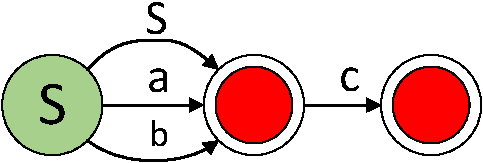
\includegraphics[width=5cm]{pictures/G2.pdf}}
				\only<2>{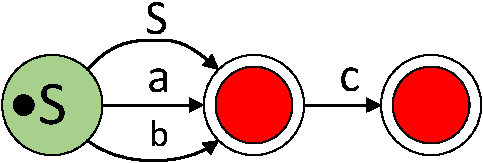
\includegraphics[width=5cm]{pictures/G2_1.pdf}}
				\only<3>{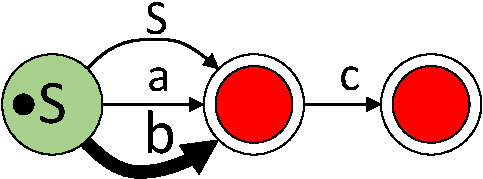
\includegraphics[width=5cm]{pictures/G2_2.pdf}}
			\end{column}
			\begin{column}{3cm}
				%\only<3>{\vspace{50pt}}
				\begin{center}
				\only<2>{
				Descriptors queue\\
				\begin{tabu}{|[3pt]c|[3pt]}
					\only<2->{$S$, 0, \dots, \dots}
				\end{tabu}
				}
				\only<3>{
					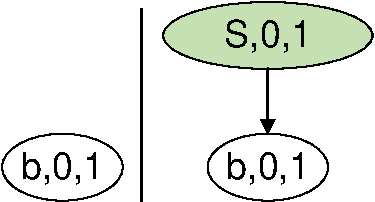
\includegraphics[width=4cm]{pictures/example_trees_auto.pdf}
				}
				\end{center}
			\end{column}
		\end{columns}
	\end{frame}
	
	\begin{frame} 
		\frametitle{Evaluation}
		\begin{center}
		\vspace{-10pt}
		Grammar $G_1$\\
		\vspace{6pt}
		$
		\begin{array}{rl}
		S =& K\ K\ K\ K\ K\ K \ | K\ a\ K\ K\ K\ K \\
		K =& S\ K\ |\ a\ K\ |\ a \\
		\end{array}
		$
		\\
		\vspace{10pt}
		RA for grammar $G_1$
		\\
		\vspace{6pt}
		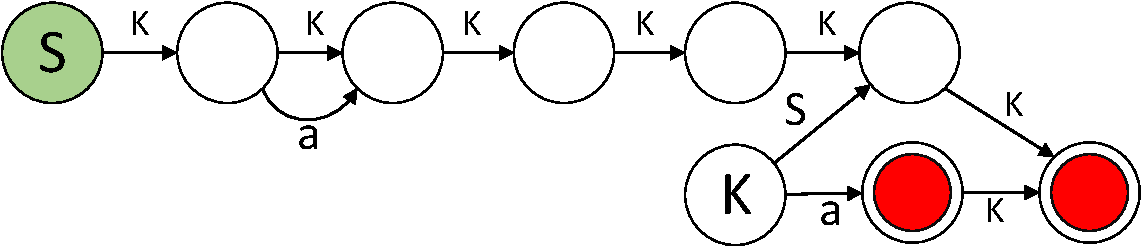
\includegraphics[scale=.5]{pictures/G1automaton.pdf}
		\\
		\vspace{7pt}
		Experiment results for input $a^{40}$
		\\
		\vspace{2pt}
		\begin{tabular}{ | c | c | c | c | c | }
			\hline
			\multirow{2}{*}[-1ex]{} &\multicolumn{3}{c|}{Memory usage} & \multirow{2}{*}[-1ex]{Time,sec} \\
			\cline{2-4}
             &  Descriptors & Stack Edges & SPPF Nodes &    \\ \hline
			Grammar  &  7,940        & 6,974      & 111,127,244 & 81 \\ \hline
		     RA &  5,830        & 4,234      & 74,292,078  & 54 \\ \hline \hline
			Ratio   &  27$\%$       & 39$\%$     & 33 $\%$ & 35 $\%$    \\ \hline
		\end{tabular}
		\end{center}
	\end{frame}
	
	\begin{frame} 
		\frametitle{Applicability} 
		\begin{center}
		\vspace{-40pt}
		Graph parsing: all input strings in one graph
		\begin{columns}
			\begin{column}{1cm}
			\end{column}
			\begin{column}{1cm}
				\begin{center}
				$abcd$ \\ 
				$abfd$
				\end{center}
			\end{column}
			\begin{column}{.7cm}
				\\
				$ \Longrightarrow $
			\end{column}
			\begin{column}{6cm}
			
\includegraphics[width=6cm]{pictures/graph.pdf}
			\end{column}
		\end{columns}
		\vspace{40pt}
		Graph parsing results
		\begin{tabular}{ | c | c | c | c | c | }
			\hline
			\multirow{2}{*}[-1ex]{} &\multicolumn{3}{c|}{Memory usage} & \multirow{2}{*}[-1ex]{Time, min } \\
			\cline{2-4}
			             &  Descriptors & Stack Edges & Stack Nodes &   \\ \hline
			Grammar  &  21,134,080       & 7,482,789      & 2,731,529      & 02.26  \\ \hline
			RA &  9,153,352        &  2,792,330     & 839,148        & 01.25  \\ \hline \hline
			Ratio   &  57$\%$       & 63$\%$     & 69 $\%$    &  45 $\%$ \\ \hline
		\end{tabular}
		\end{center}
	\end{frame} 
	
\end{document}